\section{Anforderungen höherer Programmiersprachen}
\label{sec:anforderungen}

\paragraph{Begriffe}
\begin{itemize}
  \item \textbf{Maschinensprache}: Für Prozessor verständliche Anweisungsrepräsentation, z.B. \code{00101101001110101}
  \item \textbf{Assemblersprache}: Für Menschen verständliche Maaschinensprache, z.B. \code{add \$s2, \$s1, \$s0}
  \item \textbf{Assembler}: Übersetzt Assemblersprache eindeutig in Maschinensprache
  \item \textbf{Objektcode}: Maschinenprogramm mit ungelösten externen Referenzen
  \item \textbf{Binder/Linker}: Löst ungelöste Referenzen auf, verbindet alles zu einem ausführbaren Maschinenprogramm
\end{itemize}
\begin{figure}[ht]
  \centering
  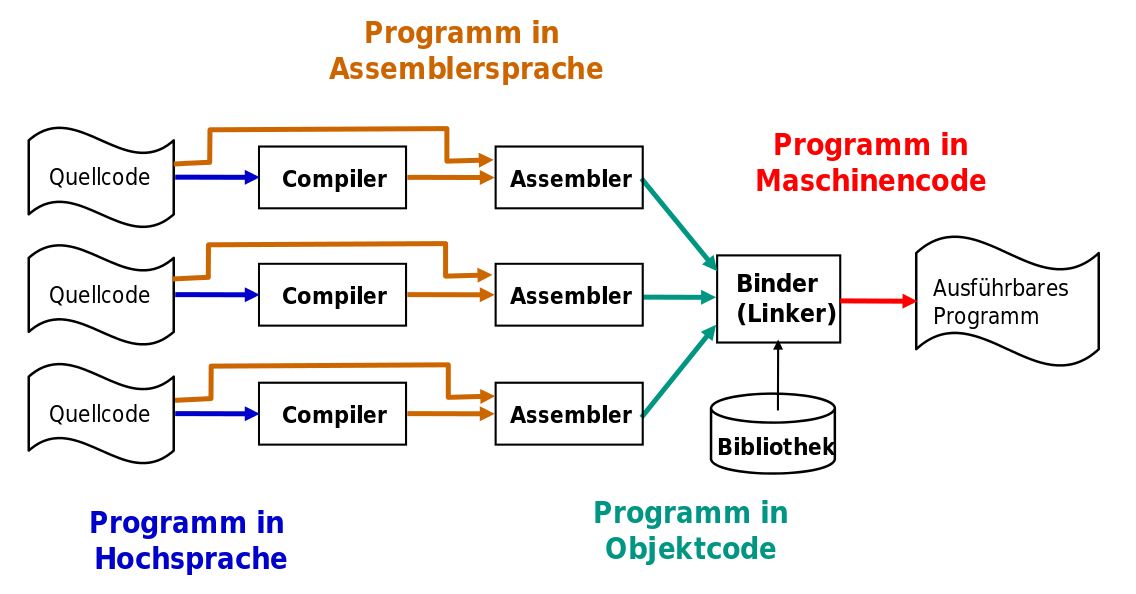
\includegraphics[width=0.33\textwidth]{QuellcodeZuProgramm}
  \label{QuellcodeZuProgramm}
\end{figure}

\paragraph{Programmiersprache C}
\begin{itemize}
  \item Zwischenstellung zwischen Assembler und Hochsprache
  \item hohe Portabilität trotz guter Architekturanpassung
  \item einfache Programmierung
  \item \textbf{Datentypen}: \code{char, int, float, double}
  \item \textbf{Kontrollstrukturen}: Entscheidungen, Schleifen, Blöcke, Unterprogramme
  \item \textbf{Zeiger} als Parameter möglich
\end{itemize}
\begin{figure}[ht]
  \centering
  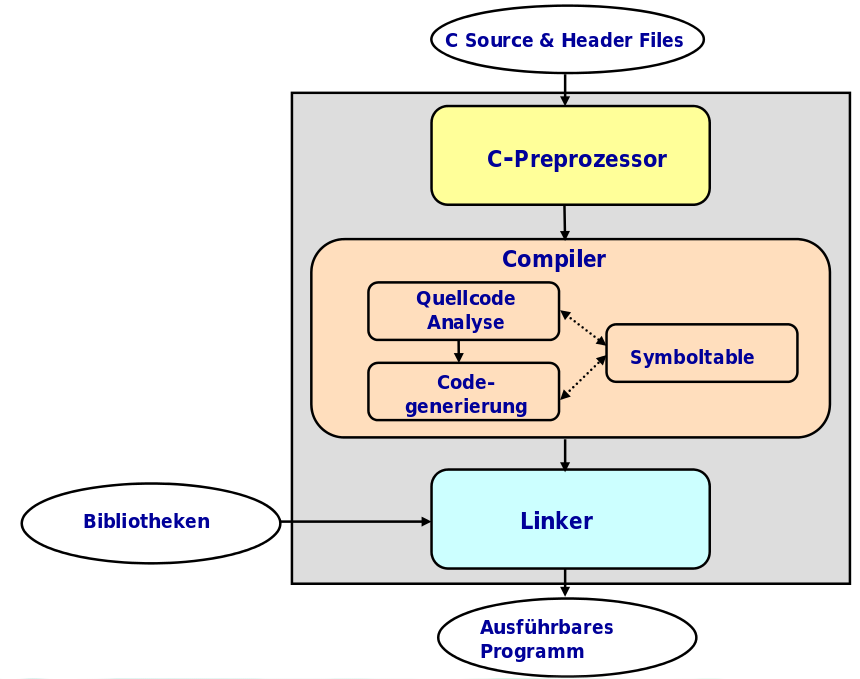
\includegraphics[width=0.33\textwidth]{CWorkflow}
  \label{CWorkflow}
\end{figure}

\paragraph{C --- Datentypen}
\begin{itemize}
  \item \textbf{\code{char}}: Ein Zeichen, meist 1 Byte
  \item \textbf{\code{int}}: Integerzahl, 2 oder 4 Byte
  \item \textbf{\code{float}}: Gleitkommazahl, meist 4 Byte
  \item \textbf{\code{double}}: Gleitkommazahl, meist 8 Byte
\end{itemize}

\paragraph{C --- Operatoren}
\begin{itemize}
  \item \textbf{\code{*}}: Multiplikation (\code{x*y})
  \item \textbf{\code{/}}: Division (\code{x/y})
  \item \textbf{\code{\%}}: Modulo (\code{x\%y})
  \item \textbf{\code{+}}: Addition (\code{x+y})
  \item \textbf{\code{-}}: Subtraktion (\code{x-y})
  \item \code{+} und \code{-} auch als Prä- und Postfix, alle auch als assign (\code{=} anhängen)
\end{itemize}

\paragraph{C --- Bit-Operatoren}
\begin{itemize}
  \item \textbf{\code{\~}}: Bitweise NOT (\code{\~x})
  \item \textbf{\code{<<}}: links schieben (\code{x<<y})
  \item \textbf{\code{>>}}: rechts schieben (\code{x>>y})
  \item \textbf{\code{&}}: bitweise AND (\code{x&y})
  \item \textbf{\code{^}}: bitweise XOR (\code{x^y})
  \item \textbf{\code{|}}: bitweise OR (\code{x|y})
  \item alle auch als Assign (\code{=} anhängen)
\end{itemize}

\paragraph{C --- Vergleichsoperatoren}
\begin{itemize}
  \item \textbf{\code{>,<}}: größer, kleiner als (\code{x>y, x<y})
  \item \textbf{\code{>=,<=}}: größergleich, kleinergleich als (\code{x>=y, x<=y})
  \item \textbf{\code{==,!=}}: gleich, ungleich (\code{x==y, x!=y})
\end{itemize}

\paragraph{C --- Spezialoperatoren}
\begin{itemize}
  \item \textbf{Auswahloperator}: \code{z = (a < b) ? a : b} (\code{z=a}, falls \code{a<b}, sonst \code{z=b<})
\end{itemize}

\paragraph{C --- Operatoren-Priorität}
\begin{figure}[ht]
  \centering
  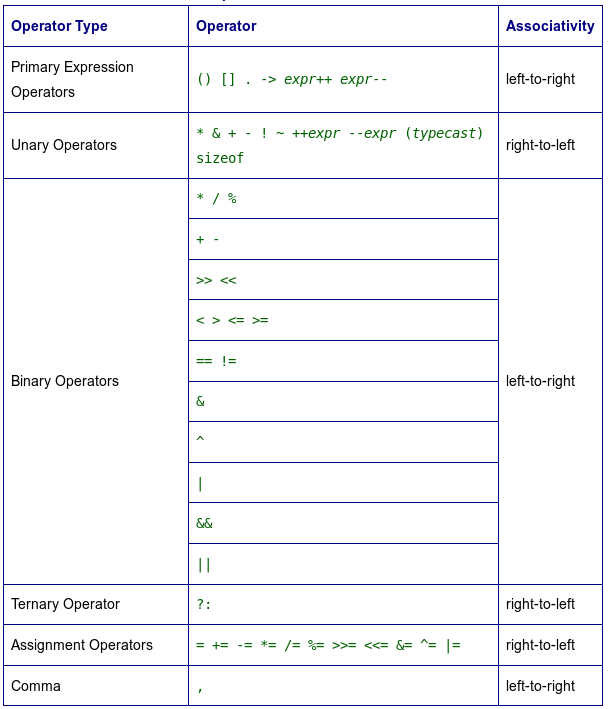
\includegraphics[width=0.33\textwidth]{Precedence}
  \label{Precedence}
\end{figure}

\paragraph{C --- Kontrollstrukturen}
\begin{itemize}
  \item \code{if (Bedigung) \{ Aktionen_if \} else \{ Aktionen_else \}}
  \item \code{switch (var) \{ case a: ... break; ... default: ... break; \}}
  \item \code{while (Bedigung) \{ ... \}}
  \item \code{for (init; Bedingung; reinit) \{ ... \}}
  \item \code{do \{ ... \} while (Bedingung)}
\end{itemize}

\paragraph{C --- Programmaufbau}
\begin{enumerate}
  \item \textbf{Präprozessor-Anweisungen}:
  \begin{enumerate}
    \item \code{#include <stdio.h>} (Bibliotheken einbinden)
    \item \code{#include \"modul.h\"} (Module einbinden)
    \item \code{#define COLOR blau} (Globale Textersetzung)
  \end{enumerate}
  \item \textbf{Globale Deklarationen/Definitionen}:
  \begin{enumerate}
    \item \code{int i;} (Deklaration)
    \item \code{int j = 13;} (Definition)
    \item \code{int fakultaet (int n);} (Funktionsprototyp)
  \end{enumerate}

  \item \textbf{Funktionen/Programmstruktur}
  \begin{itemize}
    \item \code{int fakultaet (int n) \{  ... \}}
    \item jedes Programm enthält Funktion \code{void main(...) \{ ... \}}
    \item Unterprogramm = Funktion
    \item Programmstart: \code{main} wird aufgerufen
    \item Rekursion ist zulässig
  \end{itemize}
\end{enumerate}

\paragraph{C --- Parameterübergabe}
\begin{enumerate}
  \item \textbf{Call by Value}: Normalfall, Kopie des Parameters wird an Funktion übergeben, bei Änderung keine Auswirkung beim Aufrufer
  \item \textbf{Call by Reference}: Mit Zeigern umsetzbar, selbe Speicheradresse wie Aufrufer
\end{enumerate}

\paragraph{C --- globale und lokale Variablen}
\begin{itemize}
  \item \textbf{Global}: Sind gesamtem Programm bekannt (zu vermeiden)
  \item \textbf{Lokal}: Nur in Block deklariert
\end{itemize}

\paragraph{C --- Speicherklassen}
\begin{itemize}
  \item \textbf{\code{auto}}: lokale Variablen
  \item \textbf{\code{register}}: wird in CPU-Register gespeichert, nur für zeitkritische Variablen zu verwenden
  \item \textbf{\code{static}}: statischer Speicherplatz
  \item \textbf{\code{extern}}: globale Variable
\end{itemize}

\paragraph{C --- Zeiger und Vektoren}
\begin{itemize}
  \item \textbf{Pointer}: Enthält Adresse, die auf Daten verweist
  \item \code{int* p} (\code{p} ist Zeiger auf \code{int})
  \item \code{a = 3; p = &a} (\code{p} enhält Adresse von \code{a})
  \item \code{int b = *p + 1} (\code{=4})
\end{itemize}
\begin{figure}[ht]
  \centering
  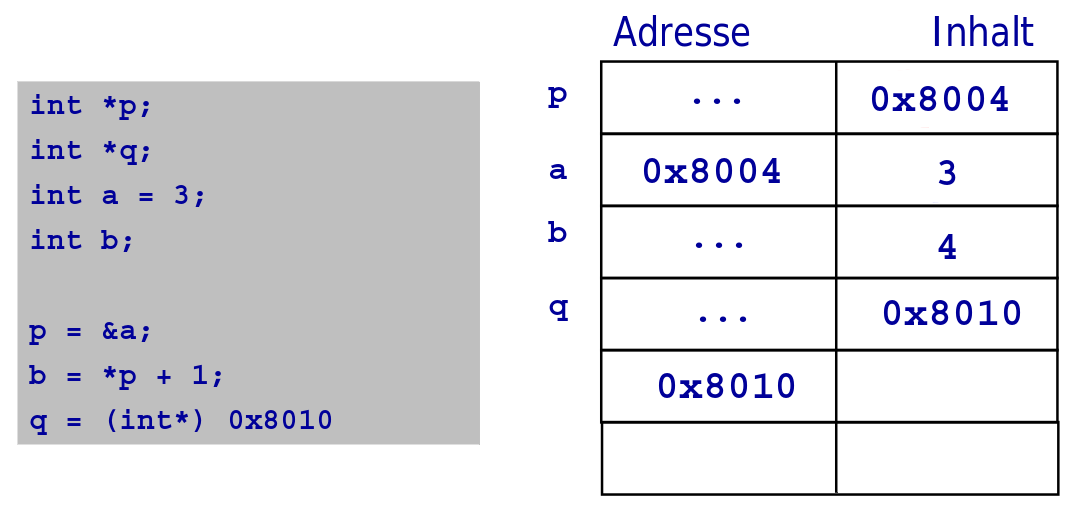
\includegraphics[width=0.33\textwidth]{Pointer}
\end{figure}